\begin{figure}[!ht]
    \centering
    \begin{subfigure}{0.49\textwidth}
        \centering
        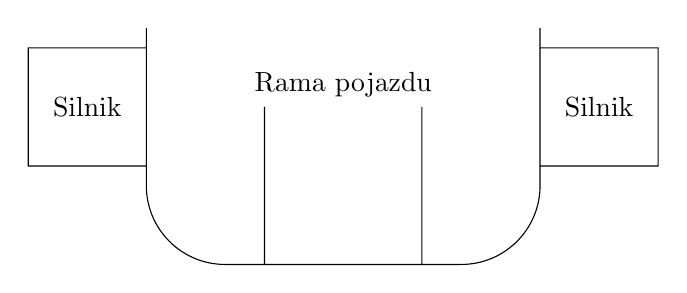
\begin{tikzpicture}
            \draw
                (0, 0) -- ++ (0, -2)
                    arc(0:90:-1)
                    -- ++ (3, 0)
                    arc(-90:0:1)
                    -- ++ (0, 2)

                (0, -0.25) rectangle node[]{Silnik} ++(-1.5, -1.5)
                (5, -0.25) rectangle node[]{Silnik} ++( 1.5, -1.5)


                (1.5, -3) --++(0, 2)
                (3.5, -3) --++(0, 2)
                (2.5, -1) node[above]{Rama pojazdu}
            ;
        \end{tikzpicture}
        \caption{Pierwotne połączenie}
    \end{subfigure}
    \begin{subfigure}{0.49\textwidth}
        \centering
        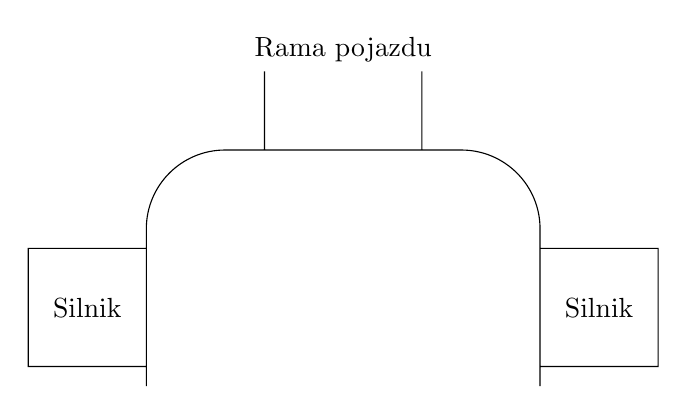
\begin{tikzpicture}
            \draw
                (0, 0) -- ++ (0, 2)
                    arc(0:-90:-1)
                    -- ++ (3, 0)
                    arc(90:0:1)
                    -- ++ (0,-2)

                (0, 0.25) rectangle node[]{Silnik} ++(-1.5, 1.5)
                (5, 0.25) rectangle node[]{Silnik} ++( 1.5, 1.5)

                (1.5, 3) --++(0, 1)
                (3.5, 3) --++(0, 1)
                (2.5, 4) node[above]{Rama pojazdu}
            ;
        \end{tikzpicture}
        \caption{Zastosowane połączenie}
    \end{subfigure}
    \caption{Schemat montażu silników}
    \label{fig:motors}
\end{figure}